\chapter{Plasmon damping as function of temperature}
\label{ch:Damping}

\begin{abstract}
This is the abstract
\end{abstract}


\section{Introduction}
Measuring temperature at the nanoscale is one of the main open challenges in
biology\cite{Yang2011a}, specially when focused into the promising fields of
photothermal\cite{Huang2006a,Hirsch2003} and photodynamic
therapy\cite{West2003}. The first normally employs small nanoparticles to
efficiently convert irradiation energy into heat in very localized
environments\cite{Ma2014a}, thus allowing to address specific
cells\cite{Hirsch2003,Huang2008}. The latter employs the nanoparticles as small
antennas, utilizing the enhanced near field to produce singlet oxygen that in
turn will induce cell apoptosis\cite{Hone2002} or to induce drug
delivery after irradiation\cite{Cheng2008}.

Successfully designing and implementing new therapies requires not only a
careful understanding of the mechanisms involved, but also needs tools to
measure and validate the hypothesis. For instance, little is reported in
literature regarding the critical temperatures needed for inducing cell
death\cite{Huang2006a}. Much less is reported regarding the effect of a single
nanoparticle in or in the vicinity of a cell.

Measuring temperature in cells has been recently subject to debate, mainly
because measurements contradict the expected thermodynamic
values\cite{Tanimoto2016,Donner2013,Yang2011a}. Therefore new
techniques that can shine light into these matters are very valuable. Moreover
these techniques should be easy to implement in existing setups and ideally
should not interfere with the environment to be measured.

Biologically relevant questions however are not the only open concerns regarding
temperature at the nanoscale. For instance the temperature of a nanoparticle in
an optical tweezer can be estimated from models\cite{Ruijgrok2011a} or by
indirect measurements. Two different approaches include looking at the
rotational diffusion coefficient\cite{Trojek2012} or by seeing
changes in a lipid bilayer standing in the vicinity\cite{Ma2014a,Urban2009}.
These methods are specific to some experiments and can't be easily generalized.

The mentioned therapies are not the only research areas where nanoparticles have
become a very promising tool. In particular gold nanoparticles have been
successfully employed as biosensors\cite{Zijlstra2012,Beuwer2015},
labels\cite{Spillane2014,Conde2013}, nanoantennas\cite{Schuller2010b,Leduc2013}
and are currently under investigation for solar energy
conversion\cite{Catchpole2008}. The main property for such broad range of
applications resides in the presence of a localized surface plasmon resonance
(LSPR) that strongly depends on the shape of the particles\cite{Zijlstra2011}.
Normally this resonance will lie between $2.34\eV$ ($530\nm$) for spheres and
the near infrared for more elongated particles.

The plasmon resonance on one hand is responsible for high electromagnetic field
enhancements near tips or protrusions\cite{Beversluis2003a,Mohamed2000}.
Because of this, nanoparticles currently are employed as nanometer size antennas
useful both for Raman scattering (SERS)\cite{Sivapalan2013} and also for
enhanced fluorescence\cite{Yuan2013,Khatua2014} experiments. On the other hand,
the plasmon resonance energy is highly sensitive to the refractive
index\cite{Prasad2015} of the medium surrounding the particles. This phenomenon
is exploited for instance in nanosensors that rely in minute changes in the
plasmon resonance to detect down to single molecules\cite{Zijlstra2012}.

The energy (or equivalently the wavelength) of the resonance is not the only
useful parameter for sensing applications. The resonance's width is also
dependent on surrounding conditions\cite{Liu2009b,Konrad2013} and therefore can
be exploited. In this work we propose the use of the FWHM of the resonance as a
parameter to measure temperature changes of the immersion medium. In order to
achieve a better understanding of the phenomenon it is important to determine
the different parameters that explain the resonance's linewidth of the plasmon.

In literature the main mechanisms involved in the description of the plasmon
resonance are electron-phonon scattering, electron-surface scattering, radiative
damping and electron-electron scattering\cite{Sonnichsen2002,Novo2006,Hu2008}.
Interband damping is neglected in this work because the resonance energies of
nanorods are low enough. Each one of the mentioned terms contributes additively
to the total plasmon damping; electron-phonon scattering however is the only one
that shows a strong dependence on temperature\cite{Liu2009b,Konrad2013}.
From the Debye model of phonons and a Fermi distribution of the conduction
electrons it is possible to calculate the damping term attributed to
electron-phonon interaction $\Gamma_{\textrm{e-ph}}$ as\cite{McKay1976},
\begin{equation}\label{eqn:broad1}
\Gamma_{\textrm{e-ph}} = 
\frac{\hbar}{\tau_0} \left[ \frac{2}{5}+4 \left( \frac{T}{\Theta_D} \right)^5
\int_0^{\Theta_D/T} \frac{z^4}{e^z - 1}\,\textrm{dz} \right]
\end{equation}

where $\tau_0 = 30\fs$\cite{Liu2009b}, $\Theta_D = 170\K$\cite{Link1999b}.  It
is important to note that this equation is valid in the case $T<\Theta_D$, in
which not all the phonon modes are occupied. For temperatures $T>\Theta_D$ and
by following a simple model for metals it is possible to simplify eqn.
\ref{eqn:broad1} into\cite{Kittel1996}
\begin{equation}\label{eqn:broad2}
\Gamma_{\textrm{e-ph}} = \lambda\pi\frac{k_\textrm{B}T}{\hbar}
\end{equation}
where $\lambda$ is a constant depending on the metal, and $k_\textrm{B}$ is
Boltzmann's constant. Equations \ref{eqn:broad1} and \ref{eqn:broad2} are
derived in the limit $E_f \gg \hbar\omega \gg k_\textrm{B}T$. For gold, 
$E_f = 5.53\eV$, and at room temperature $k_\textrm{B}T=0.026\eV$. For
nanoparticles with resonances at around $1.91\eV$ as the ones employed in this work, both
conditions are satisfied. The coefficient $\lambda$ is assumed to be a constant
of the metal, but it could also be an intrinsic property of each particle.

Previous works done at low temperatures on bulk gold\cite{McKay1976}, gold
nanorods\cite{Konrad2013} and gold bipyramids\cite{Liu2009b} showed a good
agreement of the model in equation \ref{eqn:broad1} with the experimental
results. On average it was found that the electron-phonon damping increases
with a rate of $0.1\meV/\K$ for temperatures above the Debye temperature,
independently of the geometry. Working with nanorods or bipyramids with
resonances below $2\eV$ allows to discard interband damping mechanisms.

\begin{figure}[htp] \centering
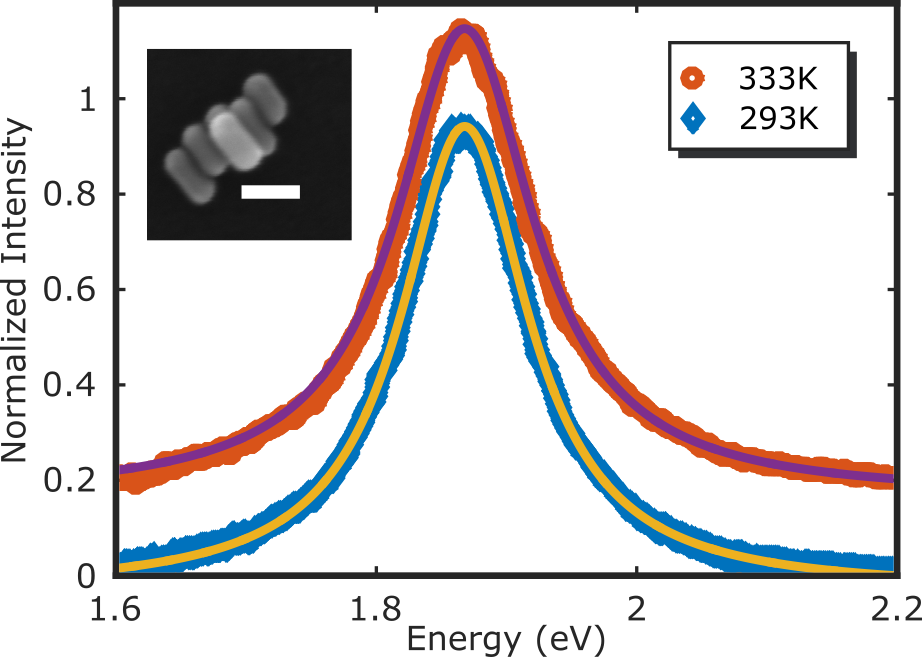
\includegraphics[width=8cm]{Chapters/05_WhiteLight/Figures/01_Spectra_Example/01_Spectra_Example.png}
\caption{Normalized scattering spectra of a single gold nanorod at $293\K$ and
at $333\K$ with corresponding lorentzian fittings. The offset between the curves is for
clarity. The FWHM increases $3.6\meV$ with a temperature change of $40\K$. The
inset shows a SEM image of the employed nanorods. The scale bar is $50\nm$.}
	\label{fig:spectra_rod}
\end{figure}

Figure \ref{fig:spectra_rod} shows white light scattering spectra of a single
gold nanorod at $293\K$ and $333\K$ with the corresponding lorentzian fits. The
plasmonic resonance centered around $1.857\eV$ is clearly visible. The FWHM of
the fit at $333\K$ is $3.6\meV$ larger than at $293\K$; this increase in width
is of about $3\%$ over a $40\K$ temperature change. The inset of the figure
shows a SEM image of the typical particles employed in this work.

Measuring the plasmonic resonance of single gold nanorods can be achieved not
only by detecting white light scattering spectra but also by exciting their
luminescence\cite{Konrad2013}. It has to be kept in mind, however, that
measuring scattering spectra benefits from the enhanced cross section at the
resonant wavelengths without being affected by the very low quantum yield of the
luminescence\cite{Yorulmaz2012}. This in turn allows to use much lower
excitation powers and shorter acquisition times.

\section{Experimental Method}
\begin{figure}[htp] \centering
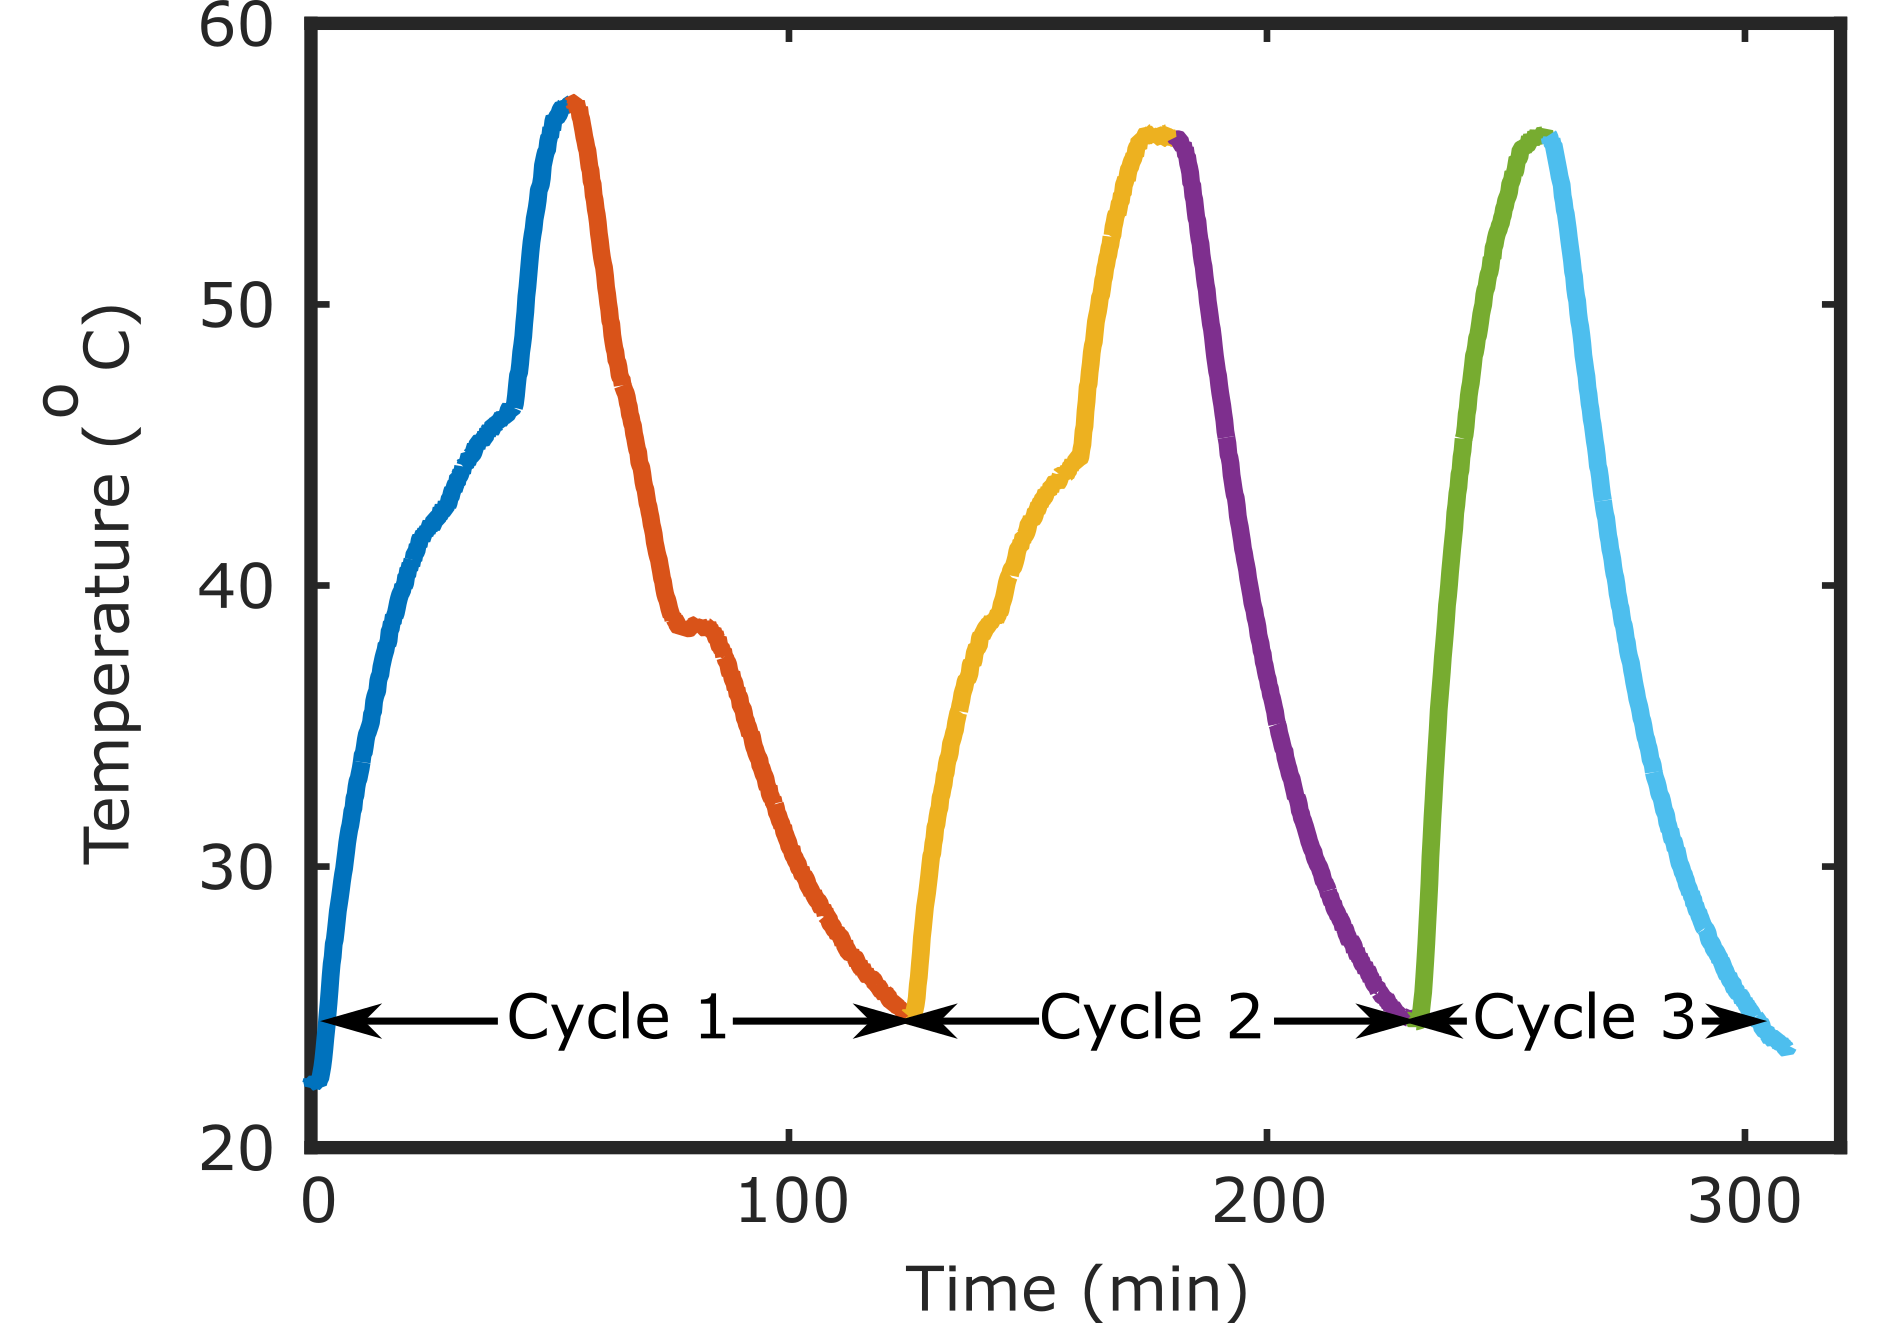
\includegraphics[width=8cm]{Chapters/05_WhiteLight/Figures/Supplementary/01_Temp_Cycle/01_Temp_Cycle.png}
\caption{Example of the temperature cycle employed for studying a single gold
nanorod. A spectra of the particle and of the background were acquired in
intervals of approximately $10\s$}
	\label{fig:temp-cycle}
\end{figure}

The experiments were performed in a home-built confocal microscope. The samples
were mounted on a flowcell that allowed to increase the temperature of the
medium up to $60\degree$. A dry objective (Olympus $60\times$ NA$0.9$) was
employed to avoid the presence of a heat sink close to the observed area. To
acquire white light scattering spectra the particles were immersed in index
matching oil, therefore achieving a dark-field configuration without changes to
the optics. Nanorods with average dimensions $20\nm\times50\nm$, as shown in the
inset of fig. \ref{fig:spectra_rod} were spin coated on top of a clean
coverslip. As a result, the number of dimers or clusters is below $1\%$ of the
observed diffraction-limited bright spots.

Spectra were recorded with an Acton $500\textrm{-i}$ spectrometer. Exposure
times were in average of two seconds. This short time was possible because the
total scattered intensity is in the order of $10^5\CPS$ with an LQNS light
source. 

Two different kind of experiments were performed. Firstly spectra of a single
nanorod were acquired continuously while varying the temperature in cycles, as
shown in Figure \ref{fig:temp-cycle}. From $19\degree$ the temperature was
increased to $60\degree$ and then freely cooled down. For the first analyzed
particle the procedure was repeated three times in order to study fluctuations
in the results given by the higher temperatures. Two more particles were studied
in the same manner, but each was subject to one thermal cycle. In every case,
after each spectrum a background was recorded in the vicinity of the particle.
 
Secondly many particles were analyzed to have better statistics on the results.
In this set of experiments, each particle's spectrum was acquired consecutively.
Also backgrounds in different regions of the sample were recorded. After the
iteration on all particles was finished, the temperature was changed to a
fixed value and the operation was repeated. In this way we have recorded the
scattering spectrum of more than $200$ particles at $9$ different temperatures
spanning from $19\degree$ to $58\degree$. The first $5$ were while increasing
the temperature, while the last $4$ when decreasing back to room temperature.

In order to compensate for the drift of the setup while changing the temperature
a special computer program to control the setup was written. In the first set of
experiments, it continuously refocused on the studied particle and triggered the
spectrometer. The same program monitored and recorded the temperature of the
flowcell by measuring the resistance of a previously calibrated Pt$100$
thermometer, placed $1\mm$ away from the observed area. Only in the first cycle
both the warming up and cooling down were done in steps, as can be seen in the
Fig. \ref{fig:temp-cycle}, in order to slowly test the procedure.

In the second experiment, a reference particle was used for compensating the
drift while changing temperature; the relative positions of the other particles
were calculated accordingly. In every case an automatic refocusing procedure was
applied before triggering the spectrometer, ensuring the correct positioning of
the desired particle in the center of the beam. With this procedure,
approximately $80$ particles can be studied at $9$ different temperatures every
under $6$ hours. Measuring the local temperature in the vicinity of the
particles is important since the PID loop used to control the flowcell
temperature can have drifts of up to $4\degree$.

\section{Results}
\begin{figure}[htp] \centering
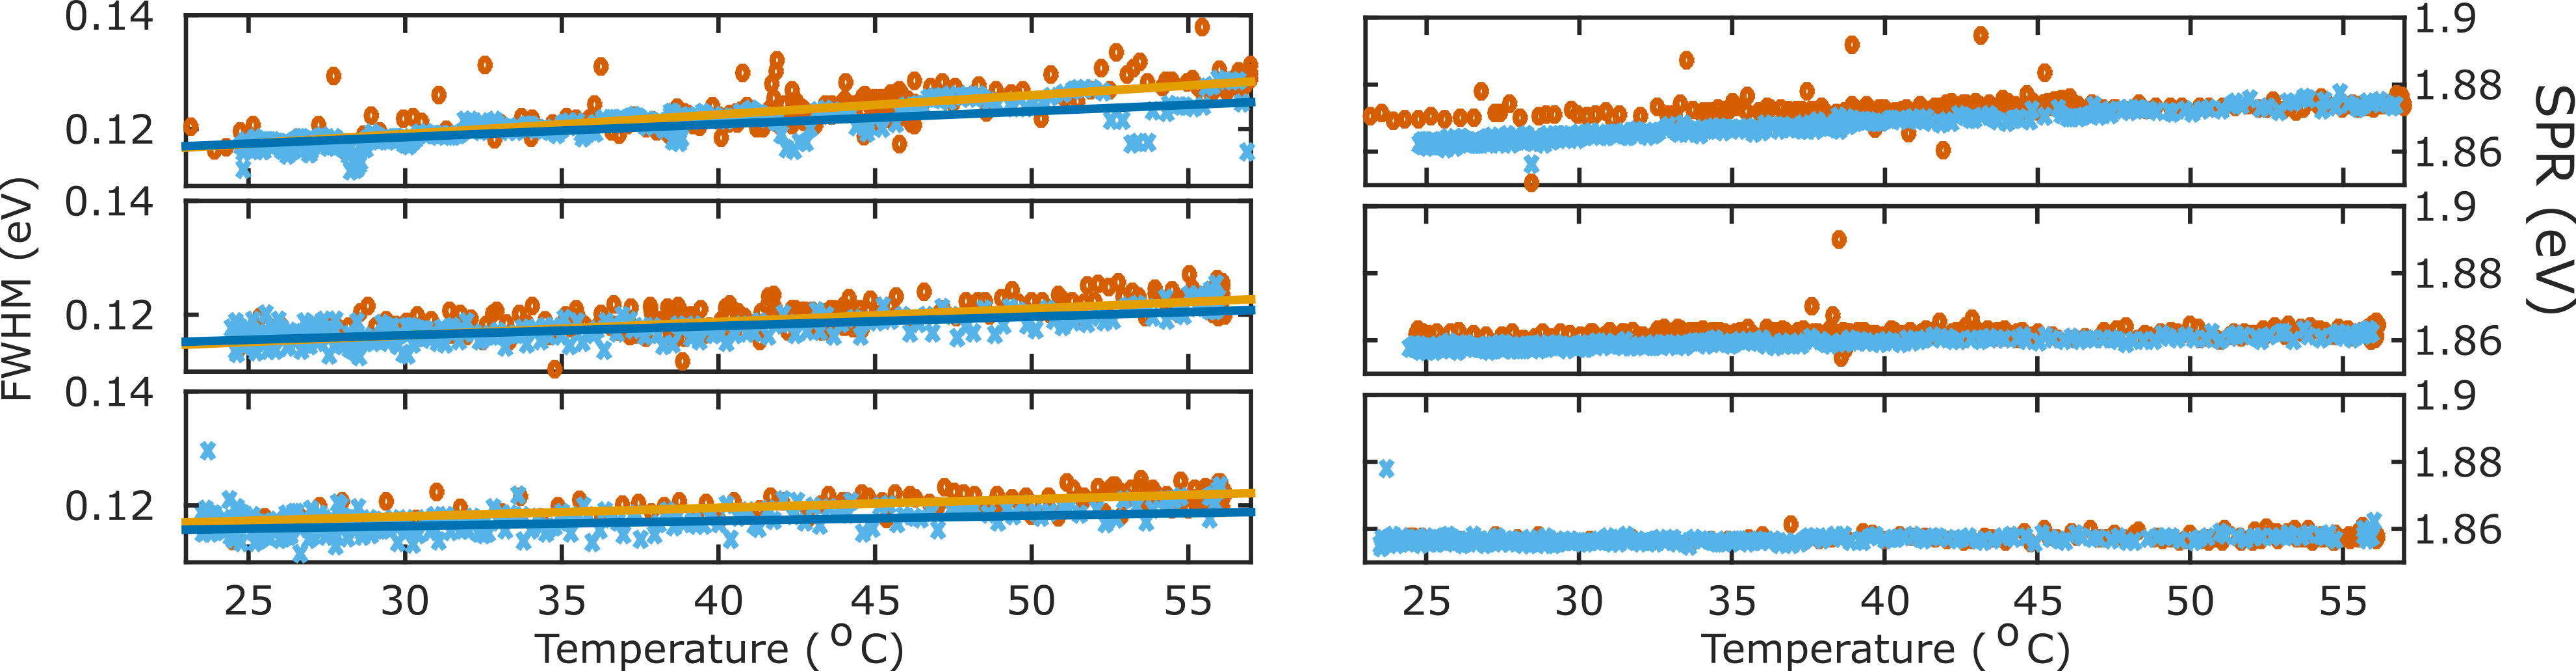
\includegraphics[width=17cm]{Chapters/05_WhiteLight/Figures/02_One_Pcle/02_One_Pcle.png}
\caption{Plasmon width (left) and resonance energy (right) for one particle at
varying temperatures. From top to bottom, each plot represents a thermal cycle,
going from room temperature to $60\degree$ (red circles) and cooling down
afterwards (blue crosses). It can be seen that after the second cycle there is
no variation of the plasmon resonance but the width increases with temperature.}
	\label{fig:one_pcle}
\end{figure}

The particle shown in Figure \ref{fig:spectra_rod} was analyzed while
continuously changing the temperature of the flowcell as described earlier. The
results are displayed in Figure \ref{fig:one_pcle} where the left column shows
the plasmon width while the right column the resonance position as function of
temperature. Each row in the figure corresponds to every temperature cycle in
Fig. \ref{fig:temp-cycle}, the first cycle on top and the last at the bottom.
The red circles correspond to the temperature increase part of the cycle, while
the blue crosses to the decreasing.

In Fig. \ref{fig:one_pcle} it is possible to observe that during the first cycle
there is a linear relationship between the plasmon resonance's width and
temperature. In this cycle the plasmon broadens at a rate of $0.34\meV/\K$.
However the resonance energy also shifts with temperature, going from $1.869\eV$
at room temperature to $1.877\eV$ at $58\degree$. More strikingly, when cooling
down the resonance energy diminishes to $1.862\eV$. During the second cycle the
broadening of the resonance is slightly less pronounced, at a rate of
$0.23\meV/\K$. The plasmon resonance even if significatively more stable than
during cycle $1$, also shows a red shift while cooling down, reaching a value of
$1.857\eV$. During the third cycle the broadening of the plasmon shows a rate of
$0.15\meV/K$ while the resonance does not depend on temperature and is stable
around $1.856\eV$.

The results of the linear fittings of the FWHM of the plasmon while changing
temperature are summarized in table \ref{table-results}. The values correspond
to the slope of the line for the increasing and the decreasing part of the cycle
separately. The first cycle shows the maximum slope of $0.34\meV/\K$, while the
cooling down of the third cycle the minimum at a rate of $0.09\meV/\K$. This
last value is in good agreement with the expected broadening rate of
$0.1\meV/\K$ reported earlier\cite{Liu2009b,Konrad2013} and expected from bulk gold
measurements. However the changes in the resonance energy have to be addressed
independently.

Normally plasmon shifts are related to changes in the refractive index of the
medium surrounding the nanoparticles. This phenomenon is used, for instance, in
photothermal imaging\cite{Berciaud2006,Gaiduk2010b} or in
biosensors\cite{Zijlstra2012} as described in the Introduction. The fact that in
the first cycle there is a non-reversible plasmon shift implies that either the
medium or the surface of the particle (or both) changed in a permanent way after
reaching higher temperatures. This can be due to a deterioration of the
immersion oil, or to an adsorption/desorption of molecules from the particle's
surface. Discriminating from both would require further studies that are out of
the scope of this work. Thermal reshaping of the nanoparticles can be ruled out
since it would have induced a blue-shift of the
resonance\cite{Liu2009,Horiguchi2008}, while we observe an overall red-shift.
Moreover the temperatures reached in this work are much lower than the needed
for observing changes in shape of the nanorods. It is however important to note
that the plasmon broadening still occurs in the third temperature cycle when no
resonance shift is observed. Therefore the broadening is not caused by changes
in the medium but by intrinsic properties of the nanoparticles, as proposed in
the introduction.

\begin{table}
\begin{tabular}{ c | c c || c | c | c}
  Cycle & B$_i$(meV/K) & B$_d$(meV/K) & Particle & B$_i$(meV/K) & B$_d$(meV/K)\\
  \hline
  1 & 0.34 & 0.23 & 2 & 0.27 & 0.23\\
  2 & 0.23 & 0.16 & 3 & 0.08 & 0.02\\
  3 & 0.15 & 0.09 & & \\

\end{tabular}
  \caption{Summary of the results of the linear fittings for particles 1 (on
  the left). 2 and 3 (on the right). B$_i$ and B$_d$ are the results for the
  \textit{i}ncreasing and \textit{d}ecreasing part of the temperature
  cycles.}\label{table-results}
\end{table}

%Figure \ref{fig:one_pcle} shows that the plasmon broadening is a consistent
%parameter for extracting the relative temperature change of the surrounding
%medium. It has to be kept in mind that the temperatures reached are too low for
%inducing a reshaping of the particles, and the white light source
%employed is not intense enough for light-induced reshaping. Moreover thermal
%reshaping of particles induces a blue shift of the resonance (particles go from
%elongated shapes to spheres) while we observed a shift towards lower energies.

\begin{figure}[htp] \centering 
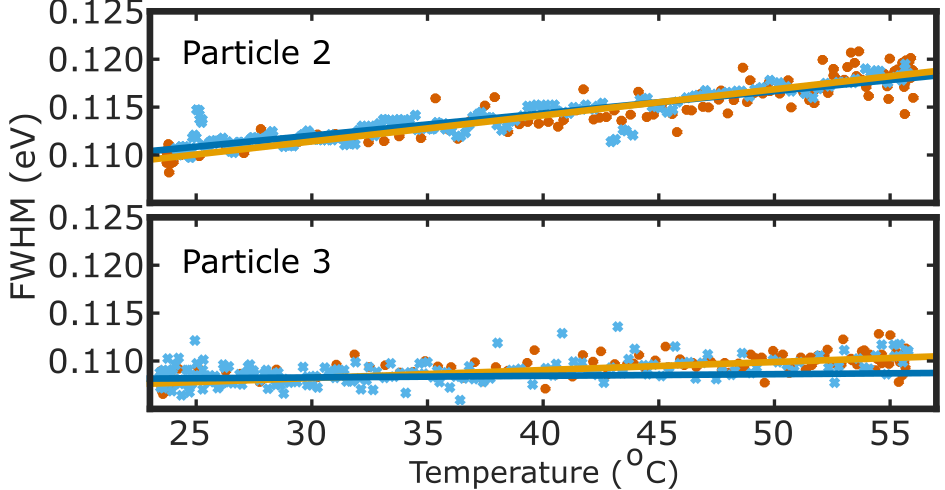
\includegraphics[width=8cm]{Chapters/05_WhiteLight/Figures/03_Two_Pcles/03_Two_Pcles.png}
\caption{Plasmon width for two particles, 
going from room temperature to $60\degree$ (red circles) and cooling down
afterwards (blue crosses). Both particles show a broadening of the plasmon
proportional to temperature, but the rates are different.}	
\label{fig:two_pcles}
\end{figure}

\begin{figure}
\centering
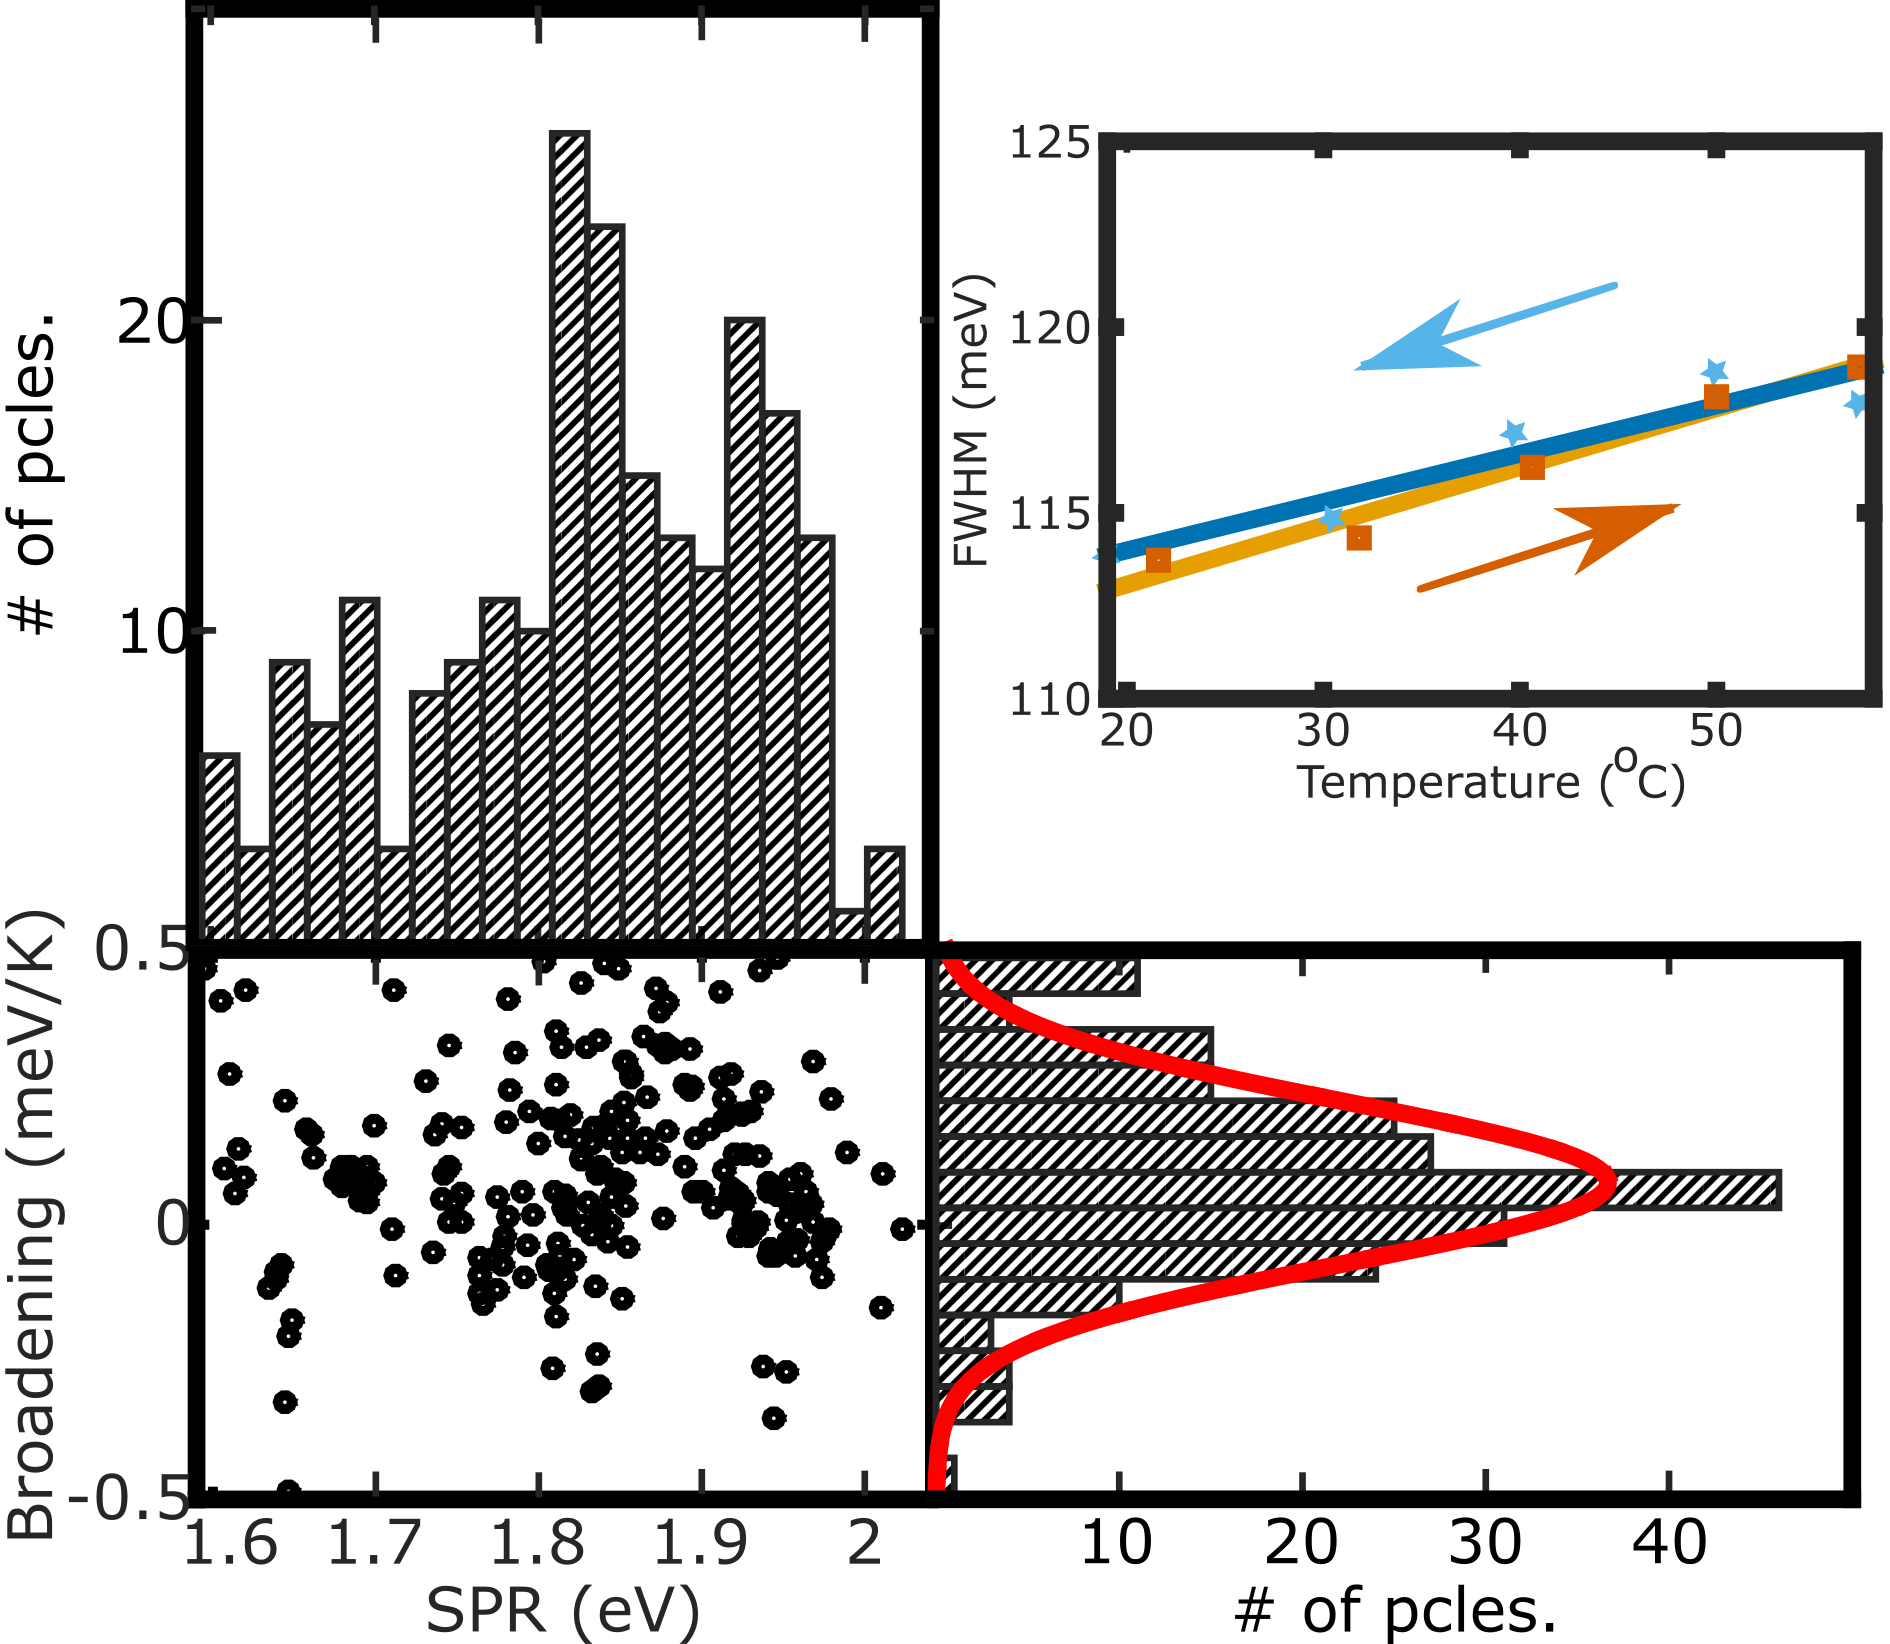
\includegraphics[width=8cm]{Chapters/05_WhiteLight/Figures/04_Many_Pcles/04_Many_Particles.png}
\caption{Plasmon broadening rates as function of initial resonance position
and corresponding histograms for $220$ different particles. Top right shows an
example of the fitting for one particle. The rates are the slopes of the
linear fits for every particle. Red squares correspond to increasing
temperatures while blue crosses correspond to the decreasing.}
		\label{fig:many-pcles}
\end{figure}

We performed the same experiment on two more particles. The measurements were
carried on right after the third cycle of particle $1$ in order to preserve the
same experimental conditions and to avoid possible changes in the immersion oil
as explained earlier. The surface plasmon resonance of both particles did not
shift during their temperature cycles. This shows that the changes induced
either on the surface of the particle or of the immersion oil at higher
temperatures have a persistence of at least few hours.

The FWHM of the resonances of these two particles are shown in Figure
\ref{fig:two_pcles}. The slopes of every fit are summarized in table
\ref{table-results} on the right columns. Particle $2$ shows a broadening rate
higher than particle $1$ while particle $3$ shows a rate lower than expected.
The heterogeneity in nanorod samples normally account for large variations in
the observables. For instance quantum yield measurements\cite{Yorulmaz2012} or
the rate of chemical etching\cite{Carattino2016} of the surface of the particles
show a broad distribution of values. To further investigate the differences
between particles and to study if there is a relationship between the broadening
rates and the plasmon resonance, we performed the same analysis on $220$
different particles.

As described earlier, we acquired the scattering spectrum of several particles
at different temperatures. The top right panel Figure \ref{fig:many-pcles} shows
the result of the procedure for one of the particles as en example. The red
squares show the FWHM of the plasmon resonance while increasing the
temperature and the blue crosses correspond to the cooling down to room
temperature. The linear fits have slopes of $0.14\meV/\K$ and $0.13\meV/\K$
respectively. Compared to the results shown in Figs. \ref{fig:one_pcle} and
\ref{fig:two_pcles}, spectra were not acquired continuously but after the
temperature was stabilized at a certain value. At each temperature spectra
of several nanorods was acquired.

From the slopes of the linear fits of all the particles analyzed it is possible
to construct the bottom left panel of Figure \ref{fig:many-pcles} and the
corresponding histograms. The particles analyzed had resonances varying from
$1.6\eV$ to $2\eV$, as shown in the top left histogram of
Fig.\ref{fig:many-pcles}. It is possible to observe that the most frequent
resonance is around $1.81\eV$. The distribution of resonance energies is also an
indication of the dispersion of shapes of the samples and is inherent to the wet
chemical synthesis methods.

The broadening rates of the $220$ studied particles are summarized in the
histogram at the bottom right. The gaussian fit of the distribution has the
center at $0.08 \meV/\K$ with a standard deviation of $0.3 \meV/\K$. This is in
good agreement with the expected broadening rate of $0.1\meV/\K$. In this
experiments care was taken in studying the particles after some thermal cycles,
in order to avoid changes in the surface plasmon resonance, as were shown in
Fig. \ref{fig:one_pcle}. 

From Figure \ref{fig:many-pcles} it is possible to discard any dependence of the
plasmon broadening rate on the plasmon's resonance position if this is kept
below the interband transition energy. The model proposed in the introduction
accounts for the broadening of the plasmon in terms of the electron-phonon
coupling in gold and can account for the average behavior observed. It is
important to note however that particles with resonances to the red normally
have narrower plasmons\cite{Sonnichsen2002}. Therefore the sensitivity of the
broadening will be higher for particles with lower resonance energies.

The distribution of rates shown in Fig. \ref{fig:many-pcles} also includes
particles that show a narrowing of the plasmon resonance while the temperature
increases. Approximately $27\%$ of the studied nanorods present a negative
broadening rate. The model of electron-phonon coupling proposed in this
work does not account for this phenomenon, nor for the different broadening
rates for different particles. It is possible that the uncertainty in the
determination of the plasmon width is responsible in part for this. The expected
plasmon resonance width change with a temperature increase of $40\K$ is of about
$4\meV$, or about $4\%$ of the FWHM of the resonance of the particles. 

\section{Conclusions}
Measuring temperature at the nanoscale is challenging. Available techniques rely
in spectral changes of fluorophores\cite{Chapman1995a} or quantum
dots\cite{Tanimoto2016,Yang2011a}. Here we show that scattering properties of
gold nanoparticles can also be used as temperature sensors. One of the main
advantages is that the scattering cross section of gold nanoparticles is in the
order of $10^3\nm^2$, and therefore the powers needed for measuring the spectrum
as well as the integration times can be low.

Electron-phonon coupling in gold is one of the parameters responsible for
the broad plasmonic resonance of nanoparticles. This is also the only
parameter that depends strongly on temperature and can be modeled with a
simple linear relation for temperatures above the Debye temperature. It is
therefore expected that the plasmon width depends linearly on temperature as was
shown in this work. 

Particles studied in detail, acquiring continuously spectra while increasing
and decreasing the medium's temperature showed a broadening of their resonances
with various rates. We have also shown that the resonance energy changes with
temperature and a persistent red-shift is observed. This is attributed to
changes in the refractive index of the medium surrounding the particles, either
due to the immersion oil changing in a non reversible way or to some
modification of the surface chemistry of the particles (for instance because
of adsorption of molecules present in the oil).

To investigate the differences in the broadening rates observed from particle to
particle and a possible relationship of these rates with the resonance position,
spectra of more than $200$ nanorods were studied. It was found that the
broadening rates have a distribution centered around $0.08\meV/\K$, while the
value expected from bulk measurements is $0.1\meV/\K$\cite{McKay1976}. The
standard deviation of the distribution of rates is $0.3\meV/\K$.

The model proposed in this work cannot account for the distribution of rates
observed. However it has to be noted that when working with gold nanoparticles,
the distribution of values of selected quantities can be of up to one order of
magnitude. For example, quantum yield measurements\cite{Yorulmaz2012}, surface
chemistry\cite{Carattino2016}, plasmon induced reactions\cite{Osinkina2013} are
some of the examples of the high variability observed from particle to particle.
This variability also makes important single-particle studies, since many of the
phenomena can be hidden in bulk measurements\cite{Link1999b}.

With the measured average broadening rate, reaching sensitivities of $1\K$ imply
detecting changes in the plasmon width of $0.08\meV$, less than $0.1\%$ of the
total width. The error in the fitting of the scattering spectrum is mainly given
by the amount of light collected. Longer exposure times can lead to lower errors
and therefore higher sensitivities. On the other hand, detecting several
particles at the same time can lead to increasing the temperature sensitivity.

\references{Chapters/05_WhiteLight/WhiteLight}
